\documentclass{beamer}

\usetheme{Singapore}

\usepackage{float}
\usepackage{multimedia}
\usepackage{color}
\usepackage{color}
\definecolor{DarkBlue}{rgb}{0.1,0.1,0.5}
\definecolor{Black}{rgb}{0,0,0}
\definecolor{Blue}{rgb}{0.1,0.1,0.9}
\definecolor{Red}{rgb}{0.9,0.0,0.1}
\definecolor{Green}{rgb}{0.0,0.9,0.0}
\definecolor{DeadGreen}{rgb}{0.3,0.6,0.3}
\definecolor{Brown}{rgb}{0.5,0.3,0.4}
\usepackage{polski}
\usepackage[utf8]{inputenc}
\usepackage{caption}
\usepackage{subcaption}

\title{Docker i Kubernetes w zarządzaniu projektem informatycznym}
\author{promotor: dr hab. Serweryn Kowalski}
\subtitle{Ewa Namysł}
\institute{Uniwersytet Śląski}
\date{11. października 2022}

\begin{document}

%STRONA TYTUŁOWA
\frame{
	\titlepage
}

%SPIS TREŚCI
\frame{
	\tableofcontents
	\frametitle{Spis treści}
}


\section{Cel pracy}

\frame{
	\frametitle{Cel pracy}
	\centering
	Celem pracy jest stworzenie projektu informatycznego opartego o architekturę mikroserwisów.\\
	\vspace{1em}
	Do konteneryzacji wykorzystywany jest Docker, \\natomiast proces automatyzacji umożliwia Kubernetes.
}


\section{Konteneryzacja}
\frame{
	\frametitle{Definicja konteneryzacji}
	\centering

	Konteneryzacja polega na spakowaniu aplikacji wraz z niezbędnymi bibliotekami oraz innymi zależnościami do tzw. kontenera.\\
	\vspace{1em}
	Kontenery są bardzo lekkie i przenośne, ponieważ nie zawierają pełnego systemu operacyjnego, lecz korzystają z funkcji systemowych komputera-gospodarza
}

\frame{
	\frametitle{Konteneryzacja a wirtualizacja}
	\centering

\begin{figure}
	\begin{subfigure}{.5\textwidth}
	  \centering
	  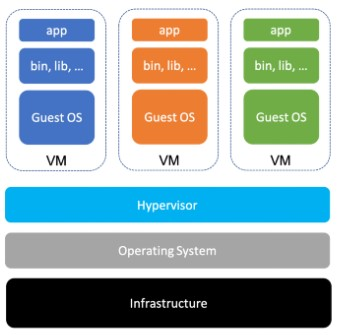
\includegraphics[width=.95\linewidth]{przyklad1.jpg}
	  \caption{wirtualizacja}
	  \label{fig:sub1}
	\end{subfigure}%
	\begin{subfigure}{.5\textwidth}
	  \centering
	  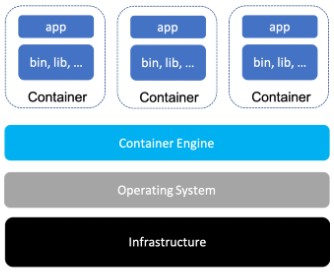
\includegraphics[width=.95\linewidth]{przyklad2.jpg}
	  \caption{konteneryzacja}
	  \label{fig:sub2}
	\end{subfigure}
\label{fig:test}
\end{figure}
}

\section{Docker}
\frame{
	\frametitle{Docker}
	\centering
	
	
\includegraphics[scale=0.2]{docker.png} \\
	\vspace{2em}
	Platforma Docker posiada rozbudowany zestaw poleceń, dzięki którym możliwe jest szybkie budowanie, modyfikowanie oraz niszczenie kontenerów. \\
	\vspace{1em}
	Możliwe jest także tworzenie plików tekstowych \textit{Dockerfile}, dzięki którym proces jest zautomatyzowany,\\
	a kontener o tej samej specyfikacji może być utworzony ponownie.
}


\frame{
	\centering
	Uruchomione kontenery działają niezależnie od siebie, są bardzo lekkie i nie wymagają tak dużej ilości zasobów w porównaniu do wirtualizacji.\\
	\vspace{1em}
	Proces ich uruchamiania i niszczenia jest bardzo szybki.\\
	Cykl życia kontenera oparty jest na zasadzie, że w razie problemów zawsze można go odtworzyć. 
}

\frame{
	\frametitle{Zalety}
	\centering
	\begin{itemize}
		\item Lekkość - w kontenerze znajdują się tylko najważniejsze funkcje systemowe.
		\item Izolacja aplikacji od siebie, jak i od systemu operacyjnego.
		\item Przenośność aplikacji - raz stworzony kontener działa wszędzie tak samo.
		\item Szybkość tworzenia nowych instancji kontenerów.
	\end{itemize}
}


\section{Orkiestracja}
\frame{
	\frametitle{Orkiestracja}
	\centering
	Orkiestracja to zautomatyzowany proces proces organizacji, koordynacji i kompleksowego zarządzania systemami komputerowymi.\\
	\vspace{1em}
	W przypadku kontenerów definicja ta ogranicza się do automatyzacji wdrażania, skalowania i zarządzania skonteneryzowanymi aplikacjami.
}


\section{Kubernetes}
\frame{
	\frametitle{Kubernetes}
	\centering
	
\includegraphics[scale=0.1]{kubernetes.jpg} \\
	\vspace{1em}
	
	Manualne zarządzanie wieloma kontenerami byłoby niemożliwe, stąd potrzeba automatyzacji w postaci Kubernetesa.\\
	\vspace{1em}
	Kubernetes umożliwia deklaratywną konfigurację i automatyzację.\\
	Za pomocą plików tekstowych jesteśmy w stanie tworzyć i modyfikować zasady działania infrastruktury monitorowanej za pomocą Kubernetesa.
}

\frame{
	\centering
	Kubernetes umożliwia:

	\begin{itemize}
		\item Balansowanie - jeśli ruch przychodzący do kontenera jest duży, Kubernetes może balansować obciążenie i przekierować ruch sieciowy, aby zapewnić stabilność aplikacji.
		\item Zarządzanie obsługą danych - zautomatyzowanie systemów do przechowywania danych.
		\item Proces tworzenia nowych kontenerów może być w pełni obsługiwany przez Kubernetesa.
		\item Automatyczne restartowanie kontenerów, które przestały działać.
		\item Zarządzanie zasobami - Kubernetes rozmieszcza kontenery na maszynach w jak najbardziej optymalny sposób.
	\end{itemize}

}


\frame{
	\frametitle{Bibliografia}
Docker - oficjalna dokumentacja. https://docs.docker.com. Dostęp:
2022-10-10.\\
	\vspace{1em}
	Kubernetes - oficjalna dokumentacja. https://kubernetes.io/docs/
home. Dostęp: 2022-10-10.\\
	\vspace{1em}
	E. Nemeth, G. Snyder, T. R. Hein, B. Whaley, D. Mackin. Unix i Linux.
Przewodnik administratora systemów. Wydawnictwo HELION, 2018. \\
	\vspace{1em}

}

\end{document}